\scanpage{4}
\figure{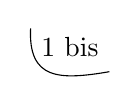
\begin{tikzpicture}[x=1cm,y=1cm]\node at (0,0) {\mspage{1 bis}};\draw[thin] (-.5,.23) .. controls (-.53,-.42) and (-.14,-.43) .. (.5,-.32);\end{tikzpicture}}
\margin{\figure{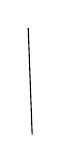
\begin{tikzpicture}\draw (0,0)--(.05,-1.35);\end{tikzpicture}}}\uline{Lemme} $A,B$ schémas abéliens sur $S$ loc. noeth, $u_\ell:T_\ell(A)\longrightarrow T_\ell(B)$.
Alors $\exists$ \uline{sous-schéma fermé} $T$ de $S$ tel que, pour tout $S'/S$ on
\inserted{ait:} $u_{\ell S'}$ provient de $u:A_{S'}\unsure{\mathbin{-}|\longrightarrow}B_{S'}$ ssi $S'$ se factorise par $T$.

Cf Inventiones 1.2 (\unsure{ou|où} démonstration \unsure{cristalline}).

\deleted{\uline{Cor} Supposons que $\forall s\in\unsure{\operatorname{Ass}^0_S|\operatorname{Ass}_S}$ \unsure{l'une des} hyp. suiv\unsure{.}
\deleted{\unsure{Ht}} \unsure{de la} \illegible{1}}
\margin{\figure{\begin{tikzpicture}\draw[thin] (0,0)--(0,-.35);\draw (0,-.5)--(.04,-1.2);\end{tikzpicture}}}\uline{Complément} De plus, pour $\forall t\in T$
tel que $\operatorname{car}k(t)=\ell$, $T$ \unsure{comprend|contient} un voisinage ouvert
\unsure{immédiat} de $t$.

\uline{Corollaire} Supposons que l'ouvert $U\subset S$ soit tel que

a) tte comp. conn. de $S$ rencontre $U$

b) $t\in S-U\Longrightarrow\operatorname{car}k(t)=\ell$.

c) $u_\ell|U$ provient de $u_U:A|U\unsure{\mathbin{-}|\longrightarrow}B|U$

Alors \deleted{\unsure{$A$}} $u_\ell$ provient de $u:A\longrightarrow B$.
\margin{donc $\Longrightarrow U\ne\varnothing$.}

\deleted{En effet, on peut supposer $S$ connexe, \inserted{Alors} \deleted{\unsure{$T$ est} \illegible{1}} \unsure{le} \illegible{2}
réunion de composantes irréductibles [dont le générique $t\in\unsure{T\cap U}$
et $t\in T\cap(S-U)$] \inserted{grâce à b)}, \deleted{\unsure{de} si $S_i$ \unsure{avait} \unsure{ou} $\unsure{\not\subset}S$
on aurait une comp. $S_i$ de $S$ telle que}
\inserted{Comme $T\ne\varnothing$, il suffit de} prouver que tte comp. irréd. de $S$ qui rencontre
$T$ est $\subset T$. Or si $S_i\cap U=\varnothing$ alors, \inserted{comme $T\supset\bar U$,} \unsure{on} aussi grâce au complément \inserted{et ailleurs}.
Donc $T\supset S_{red}$. \unsure{Alors}
Mais $T$ est \deleted{\unsure{ind}} ouvert}
$T$ est ouvert induit sur
$U$ par hyp. \inserted{c)}, et en les pts de $(S-U)\cap T$ grâce au
complément et de b). Donc $\unsure{T|\bar T}$ est un \inserted{sous-schéma} ouvert,
et comme il est fermé, c'est une réunion de
comp. connexes. Par \unsure{a)} on a donc $T=S$,
cqfd.
\mspage{3}
